\documentclass{beamer}
% or
% \documentclass[handout]{beamer}
\definecolor{LightGray}{rgb}{0.38,0.38,0.38}
\usetheme{metropolis}
\setbeamertemplate{caption}{\footnotesize\raggedright\insertcaption\par}

% ---------------------- FONTS & LANGUAGE ----------------------
% \usepackage{polyglossia} % \textenglish
% \usepackage{microtype}
% \setmainlanguage{greek}
% \setotherlanguages{english}
\def\textenglish{}

% ---------------------- OTHER ----------------------
\usepackage{adjustbox}
\graphicspath{{./images/}{./images/graphs/}}
\usetikzlibrary{arrows.meta,fit,positioning}
\usepackage{minted}
\setminted{%
    autogobble=true,%
    breaklines=true,%
    frame=single,%
    framerule=2pt,%
    linenos=false%
}
\usepackage{booktabs}

% ---------------------- CUSTOM COMMANDS ----------------------
% Write in English
\newcommand{\en}[1]{\textenglish{#1}}
% project names
\newcommand{\metamodel}{\en{R4A-NAO}}
\newcommand{\projectname}{\en{r4a-nao-nlp}}
\makeatletter
\newcommand{\escapeunderscore}{\begingroup\@makeother\_\@escapeunderscore}
\newcommand*{\@escapeunderscore}[1]{#1\endgroup}
\makeatother

% ---------------------- TITLE PAGE ----------------------
\title{Αναγνώριση ενεργειών για το ρομπότ NAO σε μη δομημένη λεκτική περιγραφή}
\subtitle[Πτυχιακή Εργασία]{%
    Διπλωματική Εργασία\\
    \scalebox{0.8}{\textcolor{LightGray}{4 Ιουλίου 2019}}%
}
\date{}
\author[Ορέστης Φλώρος-Μαλιβίτσης]{Ορέστης Φλώρος-Μαλιβίτσης --- ΑΕΜ: 7796}
\titlegraphic{
    \tikz[overlay,remember picture]
    \node[at=(current page.south east), anchor=south east] {
        \raisebox{0.3cm}{
\includegraphics[height=0.4cm]{issel.pdf}}
        
\includegraphics[height=1cm]{university.png}
    };
}
\institute[Αριστοτέλειο Πανεπιστήμιο Θεσσαλονίκης]{%
    \scalebox{0.9}{Αριστοτέλειο Πανεπιστήμιο Θεσσαλονίκης}\\
    \scalebox{0.9}{Πολυτεχνική Σχολή}\\
    \scalebox{0.9}{Τμήμα Ηλεκτρολόγων Μηχανικών \& Μηχανικών Υπολογιστών}\\
    \scalebox{0.9}{Τομέας Ηλεκτρονικής και Υπολογιστών}\\
    \scalebox{0.9}{Ομάδα Ευφυών Συστημάτων και Τεχνολογίας Λογισμικού (ISSEL)}\\[5pt]
    Επίβλεψη:\\
    Ανδρέας Λ. Συμεωνίδης -- Αναπληρωτής Καθηγητής\\
    Εμμανουήλ Τσαρδούλιας -- Μεταδιδάκτορας%
}

\begin{document}
{
\setbeamertemplate{footline}{}
\frame[noframenumbering]{\titlepage}
}

\begin{frame}{Σκοπός της διπλωματικής εργασίας}
    \begin{figure}
        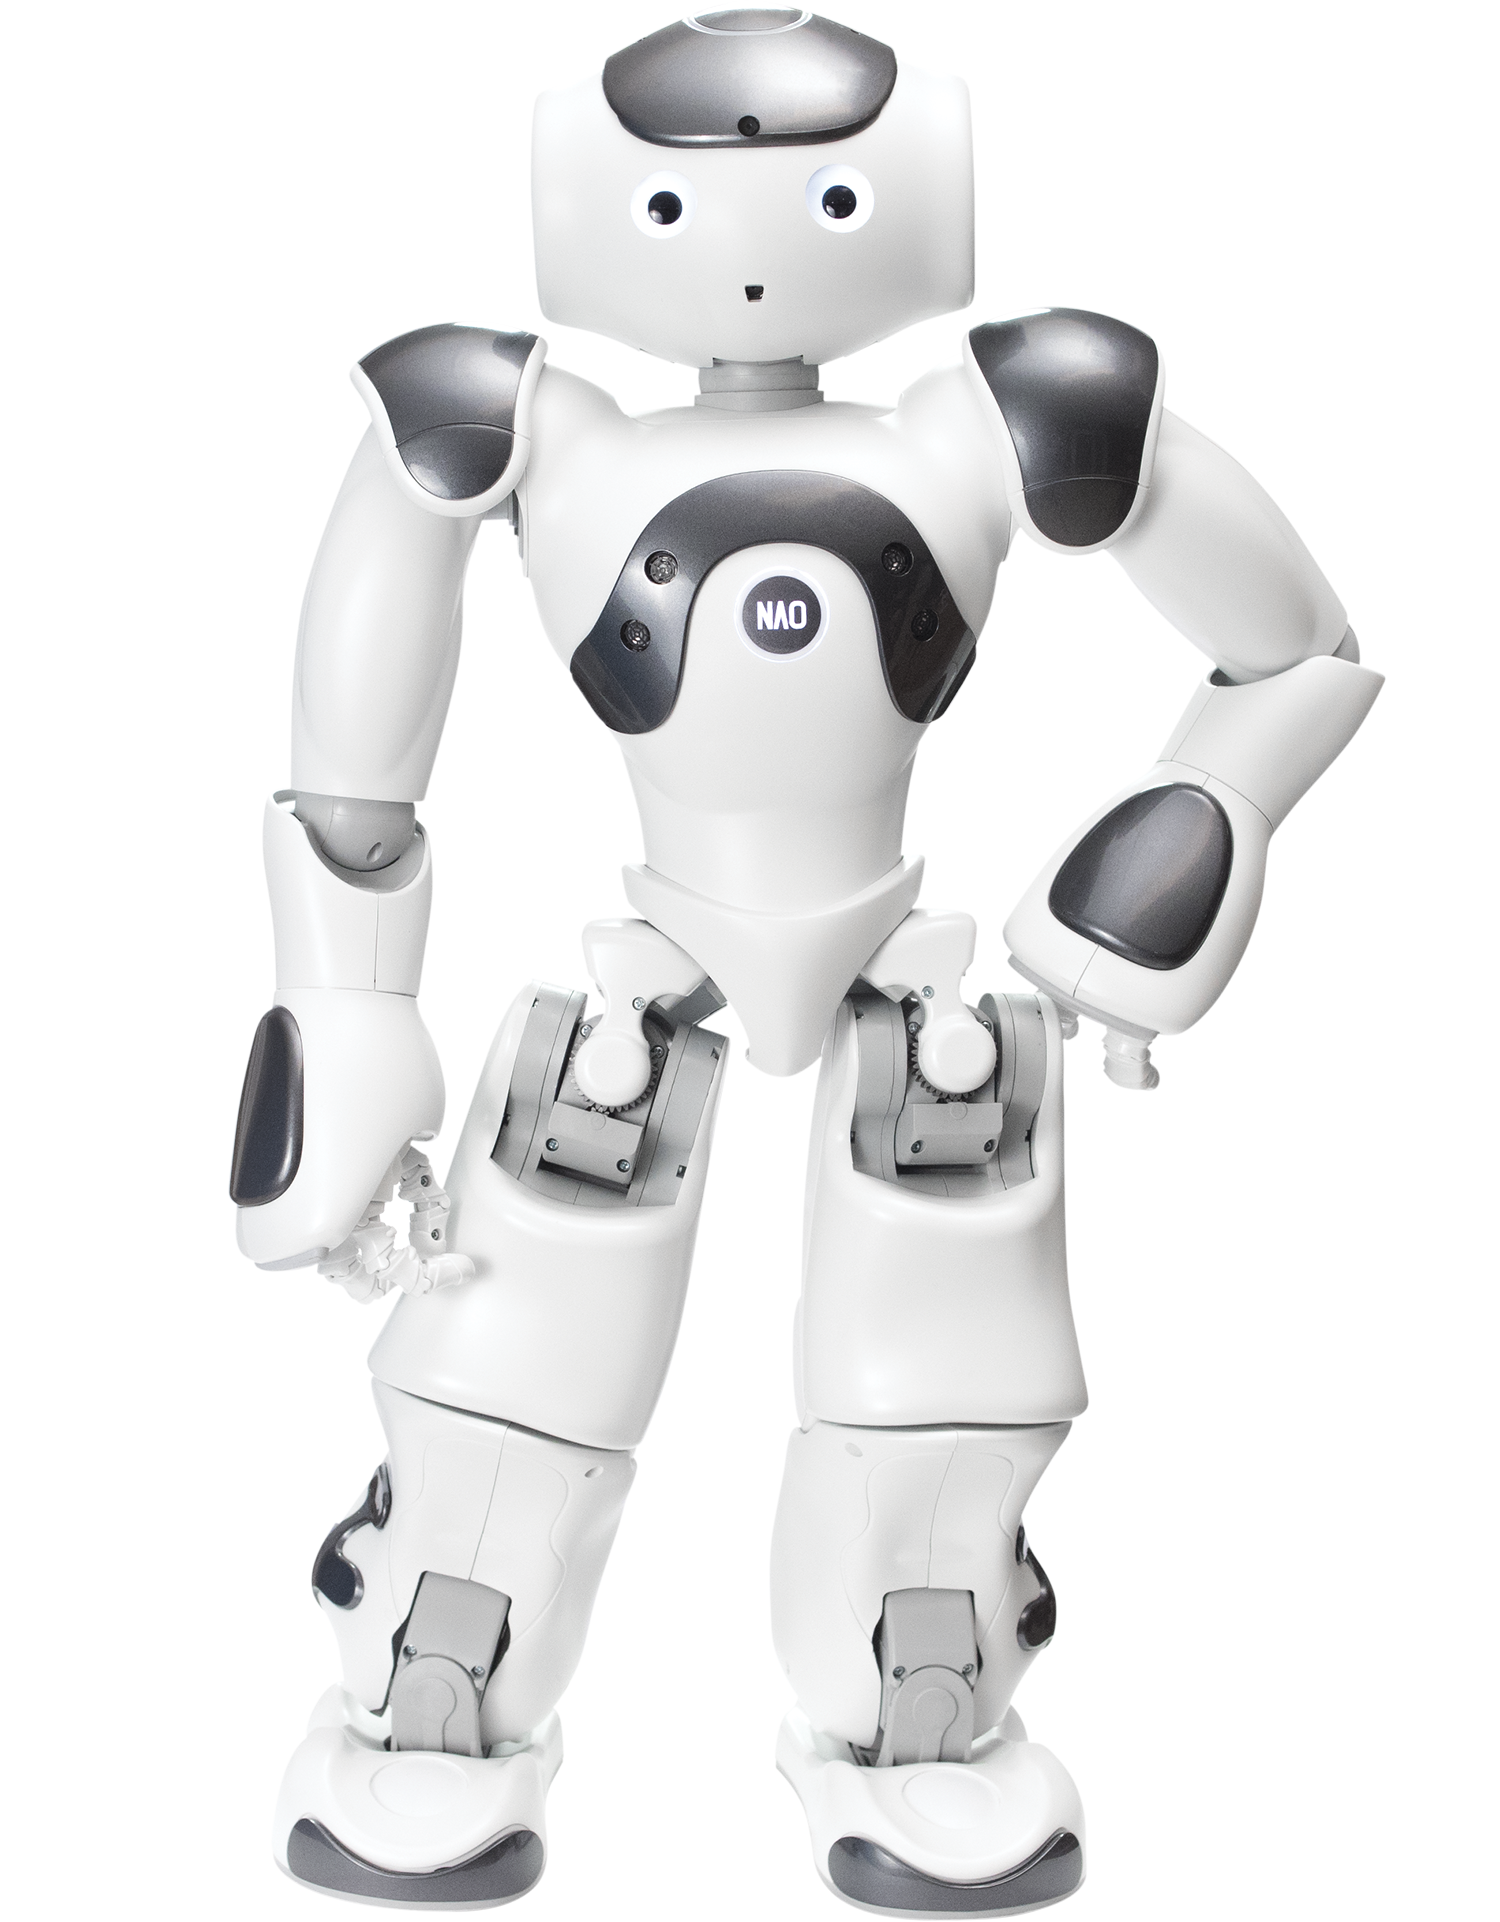
\includegraphics[height=0.4\textheight]{nao.png}
        \hfill
        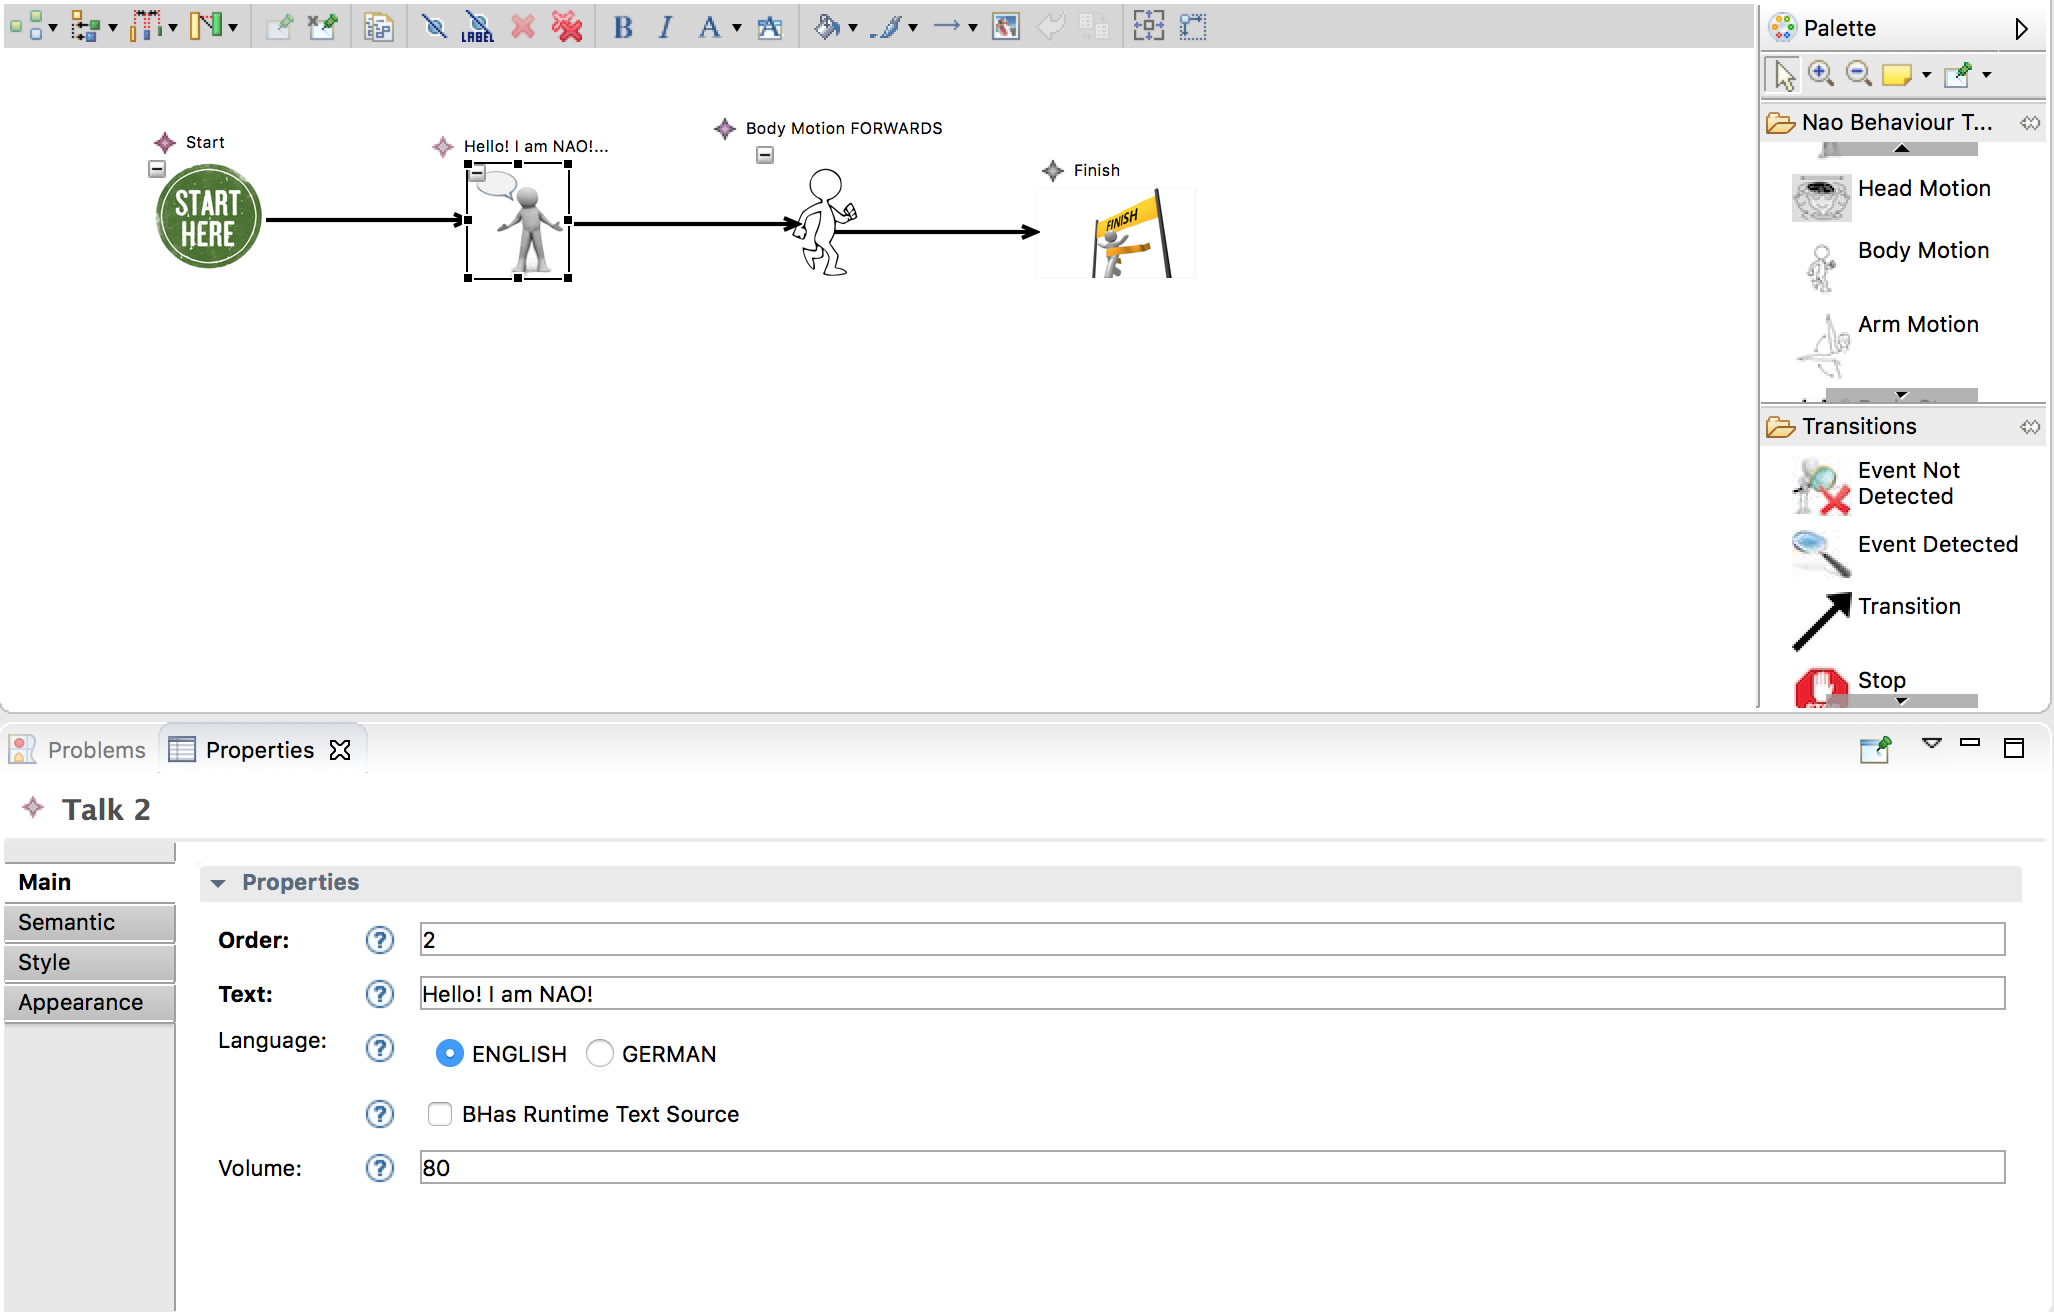
\includegraphics[height=0.4\textheight]{2-Hello-NAO-App.png}
        \caption{Το ρομπότ NAO και ένα πιθανό σενάριο χρήσης του μέσω του περιβάλλοντος του μέτα-μοντέλου \metamodel{}}
    \end{figure}
    \begin{itemize}
        \item Αναγνώριση υποστηριζόμενων ενεργειών του \metamodel{} μέσα σε κείμενο φυσικής γλώσσας
        \item Παραγωγή γράφου που περιέχει ανιχνευμένες ενέργειες και τις συνδέει με τους συνδέσμους του κειμένου
    \end{itemize}
\end{frame}

\begin{frame}{Γνώσεις που αποκτήθηκαν}
    \begin{itemize}
        \item Τρέχοντα προβλήματα που απασχολούν τον κλάδο
              \begin{itemize}
                  \item Ανάθεση σημασιολογικών ρόλων
                  \item Επίλυση συναναφορών
                  \item Αναγνώριση πρόθεσης~\& \en{slot-filling}
              \end{itemize}
        \item Ανάπτυξη \en{pipeline} μηχανικής μάθησης
        \item Εφαρμογή μοντέλων βαθιών νευρωνικών δικτύων~\& υπό συνθήκη τυχαίων πεδίων
        \item Χρήση open source βιβλιοθηκών μηχανικής μάθησης
        \item Ανάπτυξη dataset για ταξινόμηση φυσικής γλώσσας
    \end{itemize}
\end{frame}

\section{Μεθοδολογία}
\begin{frame}{Η γραφική γλώσσα \metamodel{}\hfill{}1/2}
    \begin{figure}
        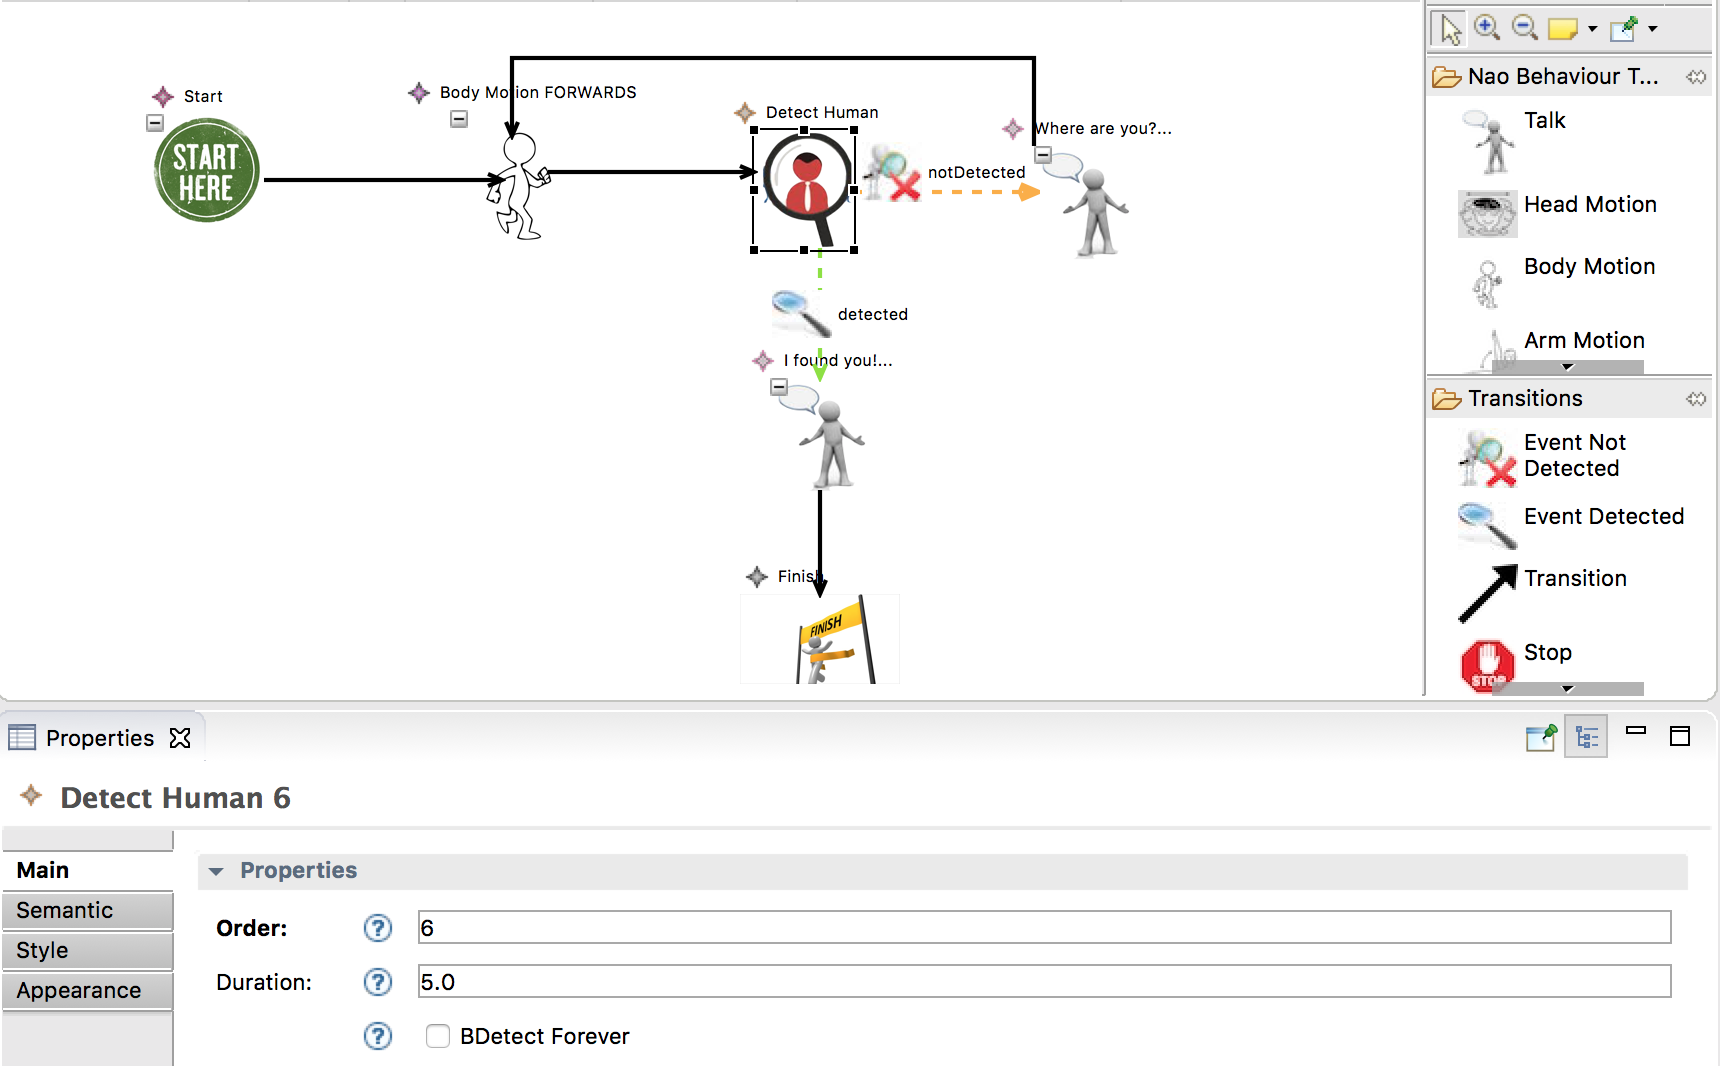
\includegraphics[width=\textwidth]{4-loop.png}
        \caption{Παράδειγμα χρήσης του \metamodel{} με βρόχο επανάληψης}
    \end{figure}
\end{frame}
{
\setbeamertemplate{frame footer}{Περαιτέρω πληροφορίες στο \url{https://r4a.issel.ee.auth.gr/nao4a/}}
\begin{frame}{Η γραφική γλώσσα \metamodel{} -- Ενέργειες\hfill{}2/2}
    \begin{table}
        \begin{tabular}{lll}
            \toprule
            Κίνησης       & Αλληλεπίδρασης & Λοιπές       \\
            \midrule
            Head Motion   & Detect Touch   & Talk         \\
            Body Motion   & Detect Human   & Dice         \\
            Arm Motion    & Detect Sound   & Sleep        \\
            Body Stance   & Detect Motion  & Turn Led On  \\
            Learn Motion  & Listen         & Turn Led Off \\
            Replay Motion & Record Sound   & Counter      \\
                          & Replay Sound   &              \\
                          & Weather Report &              \\
            % \bottomrule
        \end{tabular}
    \end{table}
\end{frame}
}

\begin{frame}[fragile]{Δεδομένα εκπαίδευσης}
    Προ-εκπαιδευμένα μοντέλα για τις περισσότερες λειτουργίες.
    Για αναγνώριση πρόθεσης~\& slot-filling:
    \begin{itemize}
        \item Χρήση βιβλιοθήκης NLU Snips για εκπαίδευση
        \item Δημιουργία dataset από το μηδέν
        \item Κάθε πρόταση περιέχει μια πρόθεση και τα σχετικά slots
        \item Επέκταση αγκίστρων \texttt{\{,\}}
    \end{itemize}
    \begin{figure}
        \inputminted[fontsize=\tiny]{text}{../data/utterances_ArmMotionOpen}
        \caption{Δεδομένα εκπαίδευσης για την πρόθεση \texttt{ArmMotionOpen}}
    \end{figure}
\end{frame}

\begin{frame}{\en{Pipeline}}
    \begin{figure}
        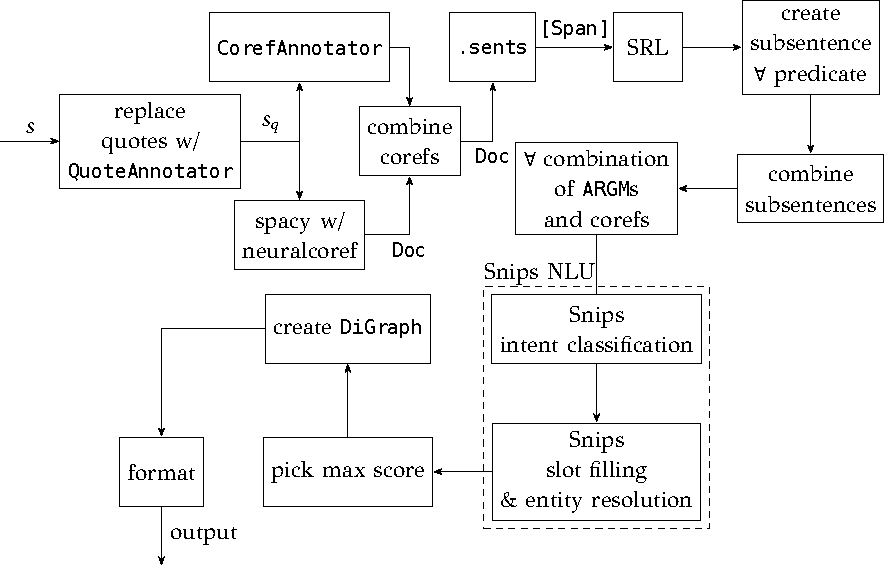
\includegraphics[width=\textwidth]{pipeline.pdf}
        \caption{Pipeline του \projectname{}}
    \end{figure}
\end{frame}

\begin{frame}{Παράδειγμα σε πρόταση}
    \begin{itemize}
        \item<1-> Open your left hand and then extend it while saying hello
        \item<2-> Συναναφορά: \textbf{it} \textrightarrow your left hand
        \item<3-> Ανάθεση σημασιολογικών ρόλων:
              \begin{enumerate}
                  \item \en{[V: Open] [ARG1: your left hand]}\\
                        \alt<3| handout:0>{%
                            \phantom{\textbf{X}}%
                        }{%
                            \alt<4| handout:0>{\textbf{Open your left hand}}{%
                                \ensuremath{\Rightarrow} \texttt{ArmMotion(armMotion=OPEN,arm=LEFT)}%
                            }%
                        }
                  \item \en{[ARGM-TMP: then] [V: extend] [ARG1: it] [ARGM-TMP: while saying hello]}\\
                        \alt<3-5| handout:0>{%
                            \phantom{\textbf{X}}%
                        }{%
                            \alt<6| handout:0>{%
                                \adjustbox{max width=\linewidth}{%
                                    \mbox{\textbf{then extend it / extend it / then extend your left hand / extend your left hand}}%
                                }%
                            }{%
                                \ensuremath{\Rightarrow} \texttt{ArmMotion(armMotion=EXTEND,arm=LEFT)}%
                            }%
                        }
                  \item \en{[V: saying] [ARG1: hello]}\\
                        \alt<3-7| handout:0>{%
                            \phantom{\textbf{X}}%
                        }{%
                            \alt<8| handout:0>{\textbf{saying hello}}{%
                                \ensuremath{\Rightarrow} \texttt{Talk(text=hello)}%
                            }%
                        }\onslide<9>{}
              \end{enumerate}
              % \item<10-> Υποπροτάσεις συμβατές μεταξύ τους -- ένας συνδυασμός
        \item[]<9-> \phantom{x}
    \end{itemize}
\end{frame}

{% Increase font size because we don't have normal text here
\setbeamertemplate{caption}{\raggedright\insertcaption\par}
\section{Αποτελέσματα}
\begin{frame}{Σενάρια χρήσης\hfill{}1/3}
    \begin{columns}[T]
        \column{0.5\textwidth}
        \begin{figure}
            \caption{Enable the leds of your chest and legs and go left}
            \begin{adjustbox}{max width=\textwidth}
                \escapeunderscore{\input{images/graphs/multi-entity-double-intent.pdf_tex}}
            \end{adjustbox}
        \end{figure}
        \column{0.5\textwidth}
        \begin{figure}
            \caption{Raise and open your left hand without extending it}
            \begin{adjustbox}{max width=\textwidth}
                \escapeunderscore{\input{images/graphs/right-node-raising.pdf_tex}}
            \end{adjustbox}
        \end{figure}
    \end{columns}
\end{frame}
\begin{frame}{Σενάρια χρήσης\hfill{}2/3}
    \begin{figure}
        \begin{columns}[onlytextwidth]
            \column{0.5\textwidth}
            \caption{Move forwards, open your left hand and turn left.
                If you see a human, close your hand.
                Else, sit down.}
            \column{0.5\textwidth}
            \begin{adjustbox}{max width=\textwidth, max height=0.9\textheight}
                \escapeunderscore{\input{images/graphs/other-coref.pdf_tex}}
            \end{adjustbox}
        \end{columns}
    \end{figure}
\end{frame}
\begin{frame}{Σενάρια χρήσης\hfill{}3/3}
    \begin{figure}
        \begin{columns}[onlytextwidth]
            \column{0.5\textwidth}
            \caption{Initially, say ``Hello everyone''.
                Then say the current date and time.
                At the same time, if someone touches you, turn the leds on.
                Finally, say ``Nice to meet you my friend''.}
            \column{0.5\textwidth}
            \begin{adjustbox}{max width=\textwidth, max height=0.9\textheight}
                \escapeunderscore{\input{images/graphs/0.pdf_tex}}
            \end{adjustbox}
        \end{columns}
    \end{figure}
\end{frame}
}

\newcommand\pro{\item[$+$]}
\newcommand\con{\item[$-$]}
\begin{frame}{Συμπεράσματα}
    \begin{itemize}
        \item Διαχωρισμός σε υποπροβλήματα
              \begin{itemize}
                  \pro Βελτίωση συνολικής απόδοσης καθώς βελτιώνονται τα μοντέλα
                  \pro Μικρότερες απαιτήσεις σε αριθμό δεδομένων
                  \con End-to-end προσέγγιση μπορεί να ενσωμάτωνε καλύτερα στατιστική συσχέτιση μεταξύ υποπροβλημάτων
              \end{itemize}
        \item Ιδέα ανίχνευσης πολλαπλών προθέσεων ανά πρόταση
              \begin{itemize}
                  \pro Δεν απαιτεί προτάσεις πολλαπλών προθέσεων στο dataset
                  \pro Επιτυχία σε σύνθετες δομές όπως ανύψωση δεξιού κόμβου
                  \con Εξαρτάται από ανάθεση σημασιολογικών ρόλων
              \end{itemize}
              \con Απαιτήσεις γραμματικά ορθών κειμένων εισόδου
              \con Δυσκολίες αν απαιτείται χρήση λογικής (συναναφορές κ.ά.)
    \end{itemize}
\end{frame}

\begin{frame}{Μελλοντική Εργασία}
    \begin{itemize}
        \item Ενσωμάτωση πληροφορίας εξωτερικού κόσμου μέσω ρομποτικών οντολογιών
        \item Χρήση συμφραζομένων από προηγούμενες προτάσεις κατά την αναγνώριση πρόθεσης
              \begin{itemize}
                  \item Απαιτεί συγγραφή περισσότερων ολοκληρωμένων σεναρίων χρήσης
              \end{itemize}
        \item Αξιοποίηση μεθόδων μεταφοράς μάθησης, end-to-end μοντέλα και ταξινόμηση πολλών ετικετών
    \end{itemize}
\end{frame}

\begin{frame}{Ευχαριστιές}
    \begin{itemize}
        \item Αναπληρωτή Καθηγητή \textbf{Ανδρέα Συμεωνίδη}
        \item Δρ. \textbf{Εμμανουήλ Τσαρδούλια}
        \item Δρ. \textbf{Χριστόφορο Ζολώτα}
    \end{itemize}
\end{frame}

\begin{frame}[standout]
    \en{Questions?}
\end{frame}

\end{document}

% vim:ts=4:sw=4:expandtab:fo-=tc:tw=120
